\section{Data treatment}
\label{sec:DataTreatment}

Having the extracted neuropil corrected fluorescence traces, F, for all of the session's time, it is also required to extract $\Delta F/F$ traces: these indicate the measured changes in fluorescence between the cell's peak stimulation times and resting state and serve as the actual data measurements to use in all of subsequent analysis.

For every ROI's trace response, the baseline fluorescence ($F_0$) was estimated by discarding the tails of the fluorescence trace distribution and taking the mean fluorescence, using a 60 s sliding window. The obtained value was then used to calculate $\Delta F/F$ traces ($\dfrac{F-F_0}{F_0}$) for each cell (figure \ref{dfoverf}, left).

Cell  $\Delta F/F$ responses are thus mostly distributed around zero, with positive tails corresponding to spike responses (for an example cell $\Delta F/F$ distribution, figure \ref{dfoverf}, right).


\begin{figure}[H] \centering 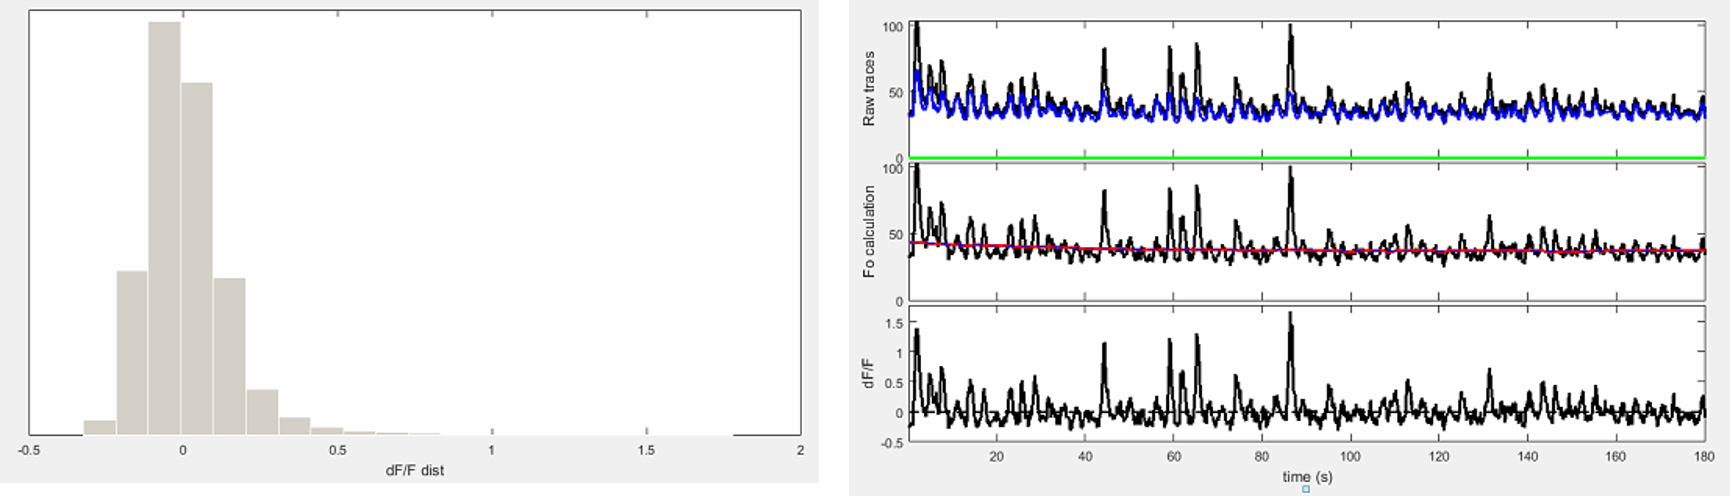
\includegraphics[width=15cm,height=15cm,keepaspectratio]{Figures/7.Results/ftraces/dFoverF.png} 
\caption{$\Delta F/F$ computation and results for an example ROI.
\newline \textbf{Left:} \textbf{Top} First 3 minutes section of raw fluorescence trace, F, for the example ROI (black trace) superimposed with the fluorescence baseline estimation trace for that ROI done by using a 60 s sliding window to discard trace's tails (blue trace); \textbf{Middle} Same fluorescence trace (black trace) superimposed with the baseline estimation value, $F_0$ (red trace), calculated as the average result of the baseline estimation trace in the top panel's blue trace, over the full session; \textbf{Bottom} $\Delta F/F$, computed as $\dfrac{F-F_0}{F_0}$.
\newline \textbf{Right:} Example ROI's $\Delta F/F$ distribution histogram. Cell's responses are mostly distributed around zero, with positive tails corresponding to spike responses.
\label{dfoverf}}
\end{figure}

Reviewing the process, we start with intrisic optical imaging on the subjects, to assess each animal's retinotopy maps and find the corresponding center field of view V1 encoding locations. 

We use two-photon imaging at that found location (with more thorough search for the center locations with the tuning protocol), and acquire brain recording sets of images of that brain's location GCaMP6s activity-related fluorescence values, for 4 different depth planes, while the subjects are shown stimuli (RF, tuning and SM protocols). 

These extracted raw images are then registered, and run through Suit2p pipeline, to select ROIs according to pixels temporal and spacial correlations in the image. These ROIs' pixels' fluorescence levels are averaged over that region and neuropil corrected. This results in raw fluorescence traces over the session's time.

With these, $\Delta F/F$ responses are computed. These are the processed data to map to the presented stimuli and use in the following analysis.

%\subsection{Receptive field mapping}
%\label{subsec:subasectionC}
%
%\subsection{Tuning mapping}
%\label{subsec:subbsectionC}
%
%\subsection{Surround modulation protocol}
%\label{subsec:subcsectionC}